\section{X-Project Architecture}
\label{sec:XPR_arc}

A Web application developed using the x-project toolkit, an x-project app, is a full stack JavaScript Single Page Application.

\subsection{Server Side}
\label{subsec:XPR_arc_serv}

On the server side, an X-Project app is based on NodeJS (see \ref{sec:TCH_nodejs}) used to create the server environment, MongoDB (see \ref{sec:TCH_mongodb}) used to storage data, and the Web framework Loopback by Strongloop (see \ref{sec:TCH_loopback}).
Loopback generates model API from the models schemas, to let CRUD operations on models. These schemas are JSON documents.


\subsection{Client Side}
\label{subsec:XPR_arc_clie}

On the client side, an X-Project app is based on HTML5 Web Components via Polymer-Project by Google.
On the top of this stack lies X-Elements a se of Polymer elements for local routing, API request, forms, lists, style and admin pages, as listed further (see \ref{sec:XPR_xel}).


\begin {figure}[h]
\graphicspath{{images/chapter_xpr/}}
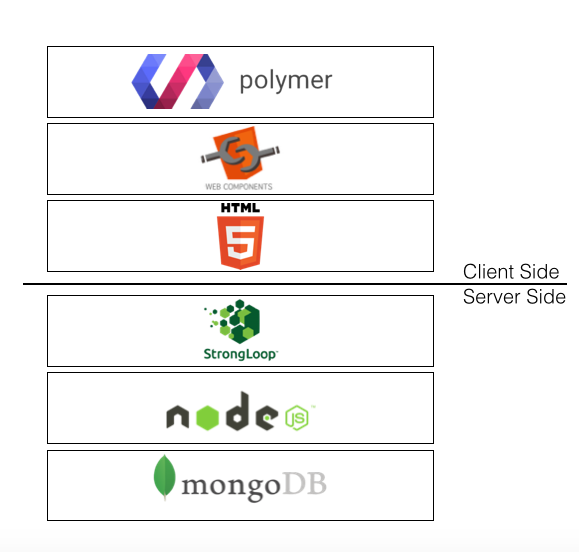
\includegraphics[width=\textwidth]{XPR_stack}
\caption{X-Project Architectural Stack }
\end {figure}